% !TeX program = latexmk
\documentclass[12pt,a4paper]{article}

% Dùng template HCMUS hiện có: giữ style, bìa, logo, header và footer.
\usepackage{hcmus-report-template}
\usepackage{tabularx,booktabs,array,titlesec,enumitem}
\setlength{\parindent}{0pt}
\newcolumntype{Y}{>{\raggedright\arraybackslash}X}

\newcommand{\coursename}{Nhập môn xử lý ngôn ngữ tự nhiên}
\newcommand{\reportname}{Đánh giá mô hình VLM và OCR trên tập dữ liệu OPRB}
\newcommand{\reporttitle}{BÁO CÁO LAB 2}
\newcommand{\studentname}{Nguyễn Quốc Nam - 24120098}
\newcommand{\teachername}{PGS.TS. Đinh Điền\\TS. Nguyễn Hồng Bửu Long}
\newcommand{\reportdate}{\today}

\lhead{\small\reporttitle}
\rhead{\small Trường Đại học Khoa học Tự nhiên - ĐHQG HCM\\\coursename}
\newcommand{\leftfooter}{}
\lfoot{\leftfooter}
\hypersetup{pdftitle={Lab 2: Đánh giá VLM và OCR trên OPRB},
            pdfauthor={Nguyễn Quốc Nam},hidelinks}

\begin{document}
\pagenumbering{arabic}
\hypersetup{pageanchor=false}
\begingroup
\setstretch{1.25}
% !TeX root = ../main.tex
\begin{titlepage}
\newcommand{\HRule}{\rule{\linewidth}{0.5mm}}
\centering

\textsc{\LARGE đại học quốc gia tphcm}\\[0.5cm]
\textsc{\Large trường đại học khoa học tự nhiên}\\[0.5cm]
\textsc{\large khoa công nghệ thông tin}\\[0.5cm]
% \textsc{bộ môn phương pháp lập trình hướng đối tượng}\\[0.5cm]

\HRule \\[0.4cm]
{ 
\huge{\bfseries{\reporttitle}}\\[0.5cm]
\large{\bfseries{Đề tài: \reportname}}
}\\[0.4cm]
\HRule \\[0.5cm]

\textbf{\large Môn học: \coursename}\\[0.5cm]

\begin{minipage}[t]{0.45\textwidth}
\begin{flushleft} \large
\emph{Sinh viên thực hiện:}\\
\studentname
\end{flushleft}
\end{minipage}
% \hfill
\begin{minipage}[t]{0.45\textwidth}
\begin{flushright} \large
\emph{Giáo viên hướng dẫn:} \\
\teachername
\end{flushright}
\end{minipage}\\[1cm]

{\large \reportdate}\\[1cm]


\includegraphics[scale=.30]{img/hcmus-logo.png}\\[1cm] 

\vfill
\end{titlepage}
	

\endgroup
\hypersetup{pageanchor=true}
\setcounter{page}{2}

% LabOCR.pdf yêu cầu dưới 4 trang A4: bìa + tối đa 2 trang nội dung.
% Không thêm trang mục lục/thành viên riêng; tác giả đã có trên bìa.
\setstretch{1.0}
\fontsize{11}{12.4}\selectfont
\setlength{\parskip}{2pt}
\setlist[itemize]{label=\textbullet,leftmargin=1.2em,topsep=2pt,itemsep=1pt,parsep=0pt,partopsep=0pt}
\setlength{\emergencystretch}{1.5em}
\setlength{\abovedisplayskip}{3pt}
\setlength{\belowdisplayskip}{3pt}
\titleformat{\section}{\normalsize\bfseries}{\thesection.}{0.4em}{}
\titleformat{\subsection}{\normalsize\bfseries}{\thesubsection.}{0.4em}{}
\titlespacing*{\section}{0pt}{5pt}{2pt}
\titlespacing*{\subsection}{0pt}{4pt}{1pt}

% !TeX root = ../main.tex
\section{Giới thiệu (Introduction)}
Báo cáo so sánh Florence-2-base (VLM) với bốn OCR nhẹ trên tài liệu bị che khuất
theo độ chính xác, độ bền vững và chi phí xử lý. Tất cả dùng trọng số pretrained,
không huấn luyện hay tinh chỉnh trên test; kết quả Florence còn thiếu.

% !TeX root = ../main.tex
\section{Thống kê dữ liệu}
\begin{itemize}
\item \textbf{Quy mô:} OPRB test~\cite{oprb} có 9.000 ảnh: 6.000 che vùng chữ
(text), 3.000 che vùng phi văn bản (nontext).
\item \textbf{Đầu vào và tham chiếu:} chỉ dùng ảnh trong
\texttt{test/\{text,nontext\}/img/}; GT (văn bản tham chiếu) từ \texttt{gt/}
chỉ dùng để chấm điểm.
\item \textbf{Phân bố:} sáu loại che được ghi ở Hình 1. Mỗi loại có 1.000 ảnh
text; nontext có 537 ảnh/loại, riêng Sim có 423 ảnh và Through\_Stamp có 429 ảnh.
\end{itemize}
Cả năm mô hình đã duyệt đủ 9.000 ảnh. Một GT chỉ có \texttt{\#\#LTFigure\#\#}
được loại chung, còn \textbf{8.999 ảnh có văn bản tham chiếu hợp lệ}
(6.000 text, 2.999 nontext). Dòng lỗi chấm điểm của PaddleOCR/Tesseract ứng với
GT này; các ảnh còn lại đều có kết quả.

% !TeX root = ../main.tex
\section{Mô tả mô hình (Model Descriptions)}
Chọn một VLM nhỏ và bốn OCR chuyên dụng để khảo sát khả năng sinh văn bản so với
pipeline phát hiện--nhận dạng. M1--M4 chạy trên một Tesla T4 của Kaggle;
M5 chạy CPU Xeon 2,00 GHz (giới hạn OpenMP 2 luồng).

\begingroup\fontsize{9.2}{10.3}\selectfont
\setlength{\tabcolsep}{3pt}\renewcommand{\arraystretch}{1.05}
\begin{tabularx}{\linewidth}{@{}l>{\hsize=0.95\hsize\linewidth=\hsize}Yl>{\hsize=1.05\hsize\linewidth=\hsize}Y@{}}
\toprule
\textbf{Mã} & \textbf{Mô hình pretrained} & \textbf{Quy mô$^*$} & \textbf{Cấu hình chạy} \\
\midrule
M1 & Florence-2-base~\cite{florence} & $\sim$230M tham số & FP16; $768^2$; \texttt{<OCR>}; 1.024 token; 3 beams; no-repeat 3-gram \\
M2 & EasyOCR 1.7.2: CRAFT + english\_g2~\cite{easyocr} & 24,55M; 93,74 MiB & FP32; canvas 2.560; greedy; batch crop 16 \\
M3 & docTR 0.11.0: DB/CRNN MobileNetV3~\cite{doctr} & 6,26M; 24,24 MiB & FP32; detector $1024^2$; crop $32\!\times\!128$; batch 128 \\
M4 & PaddleOCR 3.4.1: PP-OCRv5 mobile det + en rec~\cite{paddle} & 11,89 MiB & FP32; cạnh dài tối đa 960; batch 16; tắt xoay, unwarp, TensorRT \\
M5 & Tesseract 5.5.4: eng tessdata\_fast~\cite{tesseract} & 3,92 MiB & LSTM số nguyên; OEM 1, PSM 3; không resize; tắt học thích nghi \\
\bottomrule
\end{tabularx}
\endgroup
{\footnotesize $^*$M1 là số tham số danh định; M2/M3 đếm cả hai mạng (docTR dùng
DB MobileNetV3 Large, CRNN MobileNetV3 Small). MiB là tổng tệp trọng số đã lưu;
M5 gồm cả từ điển, không suy ra số tham số từ dung lượng. M4 dùng Paddle 3.2.0,
PaddleX 3.4.0; checkpoint/revision, hash và phiên bản được lưu trong cấu hình.\par}

% !TeX root = ../main.tex
\section{Kết quả thực nghiệm}
\subsection{Cách đánh giá}
\begin{itemize}
\item \textbf{Chuẩn hóa:} NFKC, chuyển chữ thường, gộp khoảng trắng; bỏ
\texttt{\#\#LTLine\#\#}, \texttt{\#\#LTFigure\#\#} ở GT và dự đoán.
\item \textbf{Chỉ số:} CER/WER dựa trên số phép thay thế, xóa, chèn. Precision
(P) là tỷ lệ token dự đoán khớp GT; Recall (R) là tỷ lệ token GT được nhận ra;
F1 kết hợp P và R. Token tách theo khoảng trắng, đếm số lần xuất hiện, không xét
thứ tự khi tính P/R/F1.
\item \textbf{Tổng hợp:} tính điểm từng ảnh rồi lấy trung bình đều. Thời gian xử
lý không tính tải mô hình/dữ liệu, chấm điểm hay ghi kết quả. CER/WER càng thấp
càng tốt; P/R/F1 càng cao càng tốt.
\end{itemize}

\subsection{Kết quả chung trên 8.999 ảnh}
Các tỷ lệ trong bảng dùng \%; thời gian dùng giây/ảnh.

\begingroup\fontsize{10}{11.5}\selectfont
\setlength{\tabcolsep}{4pt}
\begin{tabular*}{\linewidth}{@{\extracolsep{\fill}}lrrrrrr@{}}
\toprule
\textbf{Mô hình} & \textbf{CER}$\downarrow$ & \textbf{WER}$\downarrow$ &
\textbf{P}$\uparrow$ & \textbf{R}$\uparrow$ & \textbf{F1}$\uparrow$ & \textbf{Giây/ảnh}$\downarrow$ \\
\midrule
Florence & 61,27 & 79,33 & 53,41 & 31,69 & 38,55 & 5,597 \\
EasyOCR & 57,60 & 82,42 & 43,86 & 31,96 & 36,51 & 1,363 \\
docTR & 47,86 & 62,89 & 78,79 & 68,86 & 72,76 & 0,601 \\
PaddleOCR & \textbf{33,97} & \textbf{43,25} & \textbf{85,17} & \textbf{72,97} & \textbf{77,75} & \textbf{0,403} \\
Tesseract & 47,94 & 66,65 & 59,73 & 41,13 & 47,84 & 0,906 \\
\bottomrule
\end{tabular*}

\par\endgroup
\begin{itemize}
\item \textbf{PaddleOCR:} CER/WER thấp nhất, F1 cao nhất (77,75\%), hơn docTR 4,99 điểm.
\item \textbf{Florence:} F1 38,55\%; 1.586 đầu ra có cờ có thể bị cắt ở 1.024 token.
\end{itemize}

\clearpage
\subsection{Ảnh hưởng của vị trí và loại che khuất}
\begingroup\fontsize{10}{11.5}\selectfont
\setlength{\tabcolsep}{4pt}
\begin{tabular*}{\linewidth}{@{\extracolsep{\fill}}lrrrrrr@{}}
\toprule
& \multicolumn{3}{c}{\textbf{Che vùng chữ: 6.000 ảnh}} &
\multicolumn{3}{c}{\textbf{Che vùng phi văn bản: 2.999 ảnh}} \\
\cmidrule(lr){2-4}\cmidrule(lr){5-7}
\textbf{Mô hình} & CER & WER & F1 & CER & WER & F1 \\
\midrule
Florence & 56,03 & 77,58 & 38,69 & 71,74 & 82,83 & 38,27 \\
EasyOCR & 55,40 & 81,05 & 36,75 & 62,00 & 85,18 & 36,04 \\
docTR & 43,85 & 59,77 & 71,12 & 55,87 & 69,14 & 76,02 \\
PaddleOCR & 24,68 & 38,12 & 76,76 & 52,55 & 53,51 & 79,73 \\
Tesseract & 43,78 & 63,74 & 49,05 & 56,26 & 72,48 & 45,41 \\
\bottomrule
\end{tabular*}

\par\endgroup
PaddleOCR dẫn đầu cả hai nhóm. F1 ở nontext cao hơn text 2,97 và 4,90 điểm với
PaddleOCR và docTR, dù WER cao hơn. F1 không xét thứ tự token, còn WER có xét. Các nhóm
khác nhau về trang, nên đây là so sánh mô tả theo vị trí che.

\noindent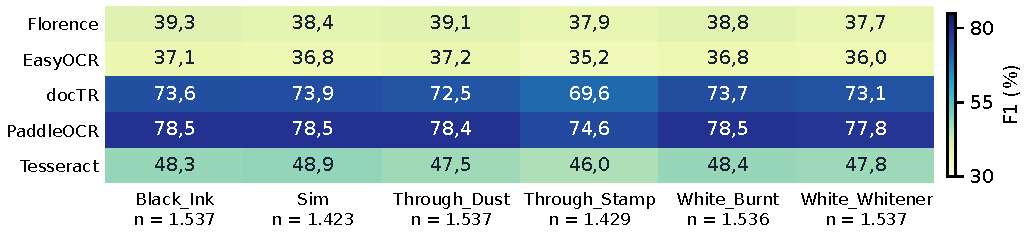
\includegraphics[width=\linewidth]{img/robustness.pdf}
{\footnotesize Hình 1. F1 theo sáu loại che khuất trên cùng tập 8.999 ảnh;
$n$ là số ảnh hợp lệ của mỗi loại.\par}
PaddleOCR có F1 cao nhất ở cả sáu loại. Through\_Stamp có F1 thấp nhất ở bốn
OCR; PaddleOCR đạt 74,58\%, thấp hơn 3,94 điểm so với Black\_Ink. Florence có
F1 thấp nhất ở White\_Whitener (37,74\%).

\subsection{Ví dụ đọc đúng và đọc sai}
Đoạn trích từ kết quả đã lưu; mã bài/trang và điểm của cả ảnh sau chuẩn hóa:

{\fontsize{10}{11.3}\selectfont
\begin{itemize}
\item \textbf{PaddleOCR -- Black\_Ink 1\%, mã 1601.04736/36:}
GT và dự đoán đều có ``Simulation Results for Parameters in FitzHugh-Nagamu Model''.
CER = WER = 0\%: toàn bộ văn bản dự đoán khớp tham chiếu sau chuẩn hóa.
\item \textbf{Tesseract -- Through\_Dust 1\%, mã 1507.03120/23:}
GT ``Mod.'' và ``24'' thành ``Mod,'' và ``os''; CER 1,63\%, WER 6,90\%.
Ví dụ cho thấy lỗi dấu câu và nhầm chữ--số.
\item \textbf{Florence -- White\_Burnt 2\%, mã 1408.3064/10:}
GT ``WIENER-WINTNER'' thành ``WIENER-WINNER''; WER 55,77\%.
Đầu ra có chuỗi số/ký hiệu dài và đạt 1.024 token: vừa có từ nhận sai vừa có cờ
có thể bị cắt.
\end{itemize}}

\subsection{Hiệu quả và giới hạn}
\begin{itemize}
\item \textbf{Chất lượng và chi phí:} PaddleOCR dùng 11,89 MiB và 0,403 giây/ảnh;
docTR dùng 24,24 MiB và 0,601 giây/ảnh trên T4, với F1 thấp hơn 4,99 điểm.
\item \textbf{Phương án CPU:} Tesseract có tệp 3,92 MiB, F1 47,84\%.
Thời gian CPU/GPU không phải phép đo trên cùng phần cứng.
\item \textbf{Giới hạn:} GT ngắn có thể làm CER/WER vượt 100\%; giữ nguyên các giá trị này.
\end{itemize}

% !TeX root = ../main.tex
\section{Kết luận}
PaddleOCR phù hợp nhất trên T4 trong thiết lập đã chạy: F1 cao nhất, tệp trọng số
nhẹ và xử lý nhanh. Tesseract là lựa chọn CPU gọn nhẹ nhưng đánh đổi bằng độ
chính xác thấp hơn.

% !TeX root = ../main.tex
\begingroup\fontsize{9}{10.3}\selectfont
\renewcommand{\refname}{Tài liệu tham khảo}
\let\originalthebibliography\thebibliography
\renewcommand{\thebibliography}[1]{%
  \originalthebibliography{#1}%
  \setlength{\itemsep}{0pt}%
  \setlength{\parsep}{0pt}%
  \setlength{\parskip}{0pt}%
}
\bibliographystyle{unsrt}
\bibliography{ref/ref}
\endgroup


% member.tex và phuluc.tex vẫn có sẵn dưới dạng tùy chọn của template,
% không nhập vào bản PDF ngắn theo yêu cầu lab.
\end{document}
